\documentclass[]{article}
\usepackage[style=numeric,backend=biber,sorting=none]{biblatex}
\usepackage{graphicx}
\usepackage{float}
\addbibresource{references.bib}

% Title Page
\title{Financial Analysis Report}
\author{Mark Paveszka}


\begin{document}
\maketitle

\newpage

\begin{abstract}
\end{abstract}

\newpage

\tableofcontents

\newpage

\section{Introduction}
\paragraph{}
As a result of modern technology, the way things are done is very different compared how it was twenty years ago. Since then everything has been speeding up, including a key area of society, namely: education. In the past fifteen to twenty years several businesses emerged to make education better and easier for both students and teachers. These businesses usually try to create software artefacts to improve some aspect of the broader field. Such software artefacts are innovative learning tools and learning management systems (LMS). One of the most well-known companies in the education technology sector is Blackboard \cite{Blackboard_UK}. They provide several applications to improve the quality of teaching in higher education, business and governmental institutes. They are mostly known for Blackboard Learn \cite{Blackboard_Learn}, which is one of the most popular learning management systems currently available on the market based on data collected by Client Stat \cite{VLE-Data} and analysed by Edutechinca \cite{VLE-2020-IMG}. The aggregation of this data is shown in Figures \ref{fig:LMS-2020} and \ref{fig:LMS-2020-6-year} which depict the market share of the most popular learning management systems in four different regions. For the purpose of this analysis only the data regarding the UK will be considered. The main competitors to Blackboard are Moodle, Canvas and Brightspace. 

\begin{figure}[H]
    \centering
    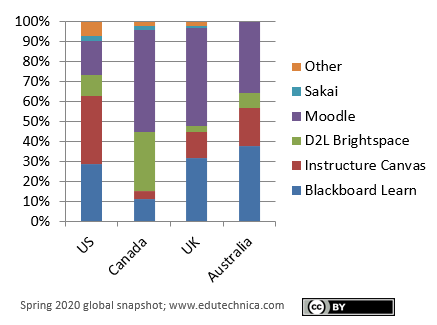
\includegraphics[width =\linewidth]{lms-vle-2020.png}
    \caption{LMS market share in 2020. \cite{VLE-2020-IMG}}
    \label{fig:LMS-2020}
\end{figure}

\begin{figure}
    \centering
    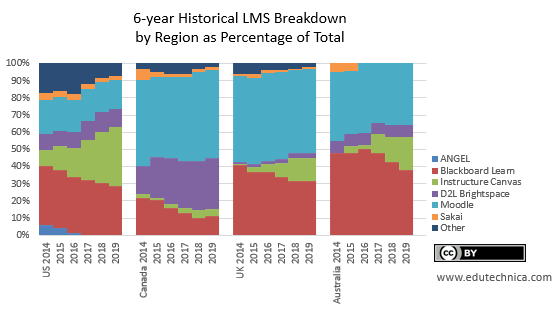
\includegraphics[width =1.2\linewidth]{lms-vle-2020-y5.png}
    \caption{6-year historical LMS data by region. \cite{VLE-2020-IMG}}
    \label{fig:LMS-2020-6-year}
\end{figure}

\paragraph{}
To obtain data some data about these companies an online tool, namely Software Advice \cite{Software-Advice} was used. This tool allowed for comparisons between the companies, which provided further insight about them. The result showed that Blackboard, Canvas and Brightspace compete in the same price range, while Moodle is cheaper to use. After examining different sources it is clear that Blackboard is not a cheap software to use \cite{Blackboard-v-Moodle}, however it provides a wide variety of features for the institutions that opt to use their system.

\paragraph{}
In 2017 the education technology sector in the UK worth around £170m \cite{Government-Strategy}. This number by 2021 is expected grow to to £3.4bn which shows that there is a lot of potential in this sector. However it is worth noting that the LMS market is part of the education technology sector and even though there will be growth it might not be that significant. Also globally there is not much change \cite{VLE-2020-IMG} in the usage of these systems compared to previous years based on Edutechnica's analysis. Globally speaking there is going to be a massive growth \cite{Markets-and-Markets} even when looking at what is projected for Europe (Figure \ref{fig:Markets-LMS}). However it is worth noting that market size of Europe will only be a small portion of the global market.

\begin{figure}
    \centering
    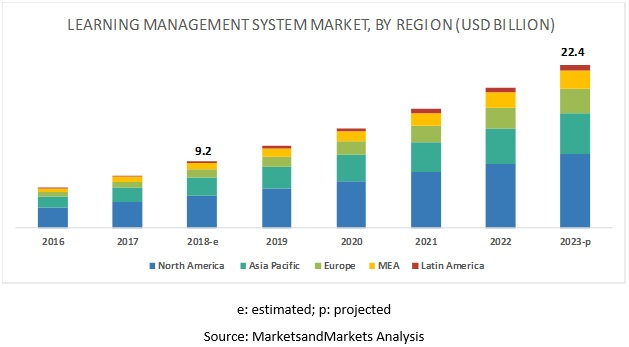
\includegraphics[width =1.2\linewidth]{learning-management-systems-market5.jpg}
    \caption{Market growth projection. \cite{Markets-and-Markets}}
    \label{fig:Markets-LMS}
\end{figure}

\newpage
\section{Financial Analysis}

\newpage
\printbibliography{}

\end{document}          
